\documentclass{standalone}
\usepackage{tikz}

\begin{document}
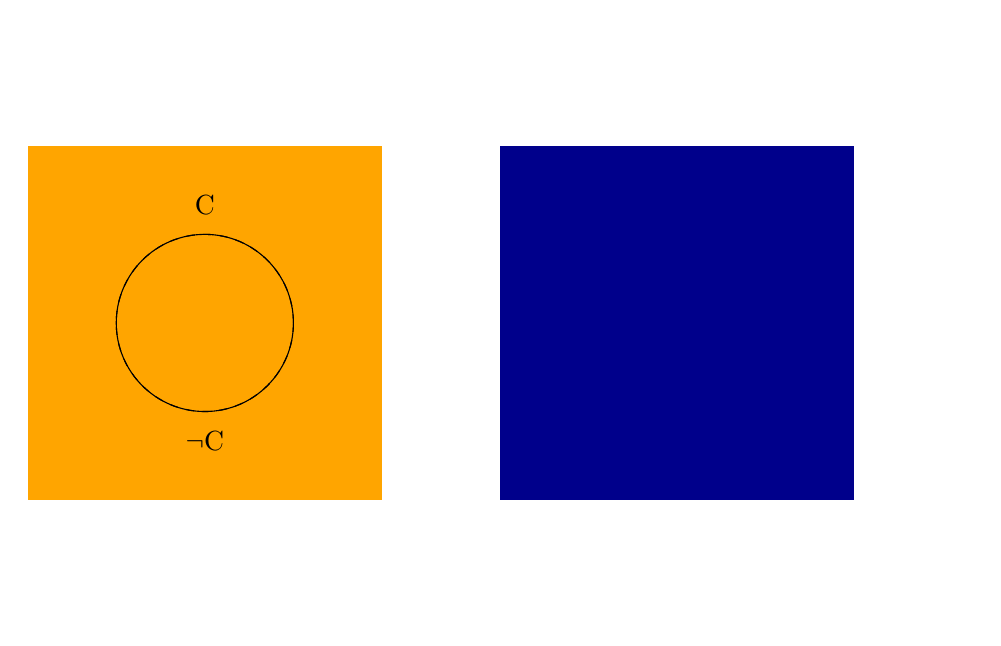
\begin{tikzpicture}[scale=1.5]

% Define colors
\definecolor{lightorange}{RGB}{255, 165, 0}
\definecolor{darkblue}{RGB}{0, 0, 139}

% Draw the white background
\fill[white] (0, -1) rectangle (8, 4);

% Draw the first rectangle (orange)
\fill[lightorange] (0, 0) rectangle (3, 3);

% Draw the second rectangle (blue)
\fill[darkblue] (4, 0) rectangle (7, 3);

% Draw the rounded corner region C
\draw[rounded corners=10pt] (1.5, 1.5) circle (0.75cm);

% Draw the region not C
\draw[dashed, rounded corners=10pt] (1.5, 1.5) circle (0.75cm);

% Add labels if needed
\node at (1.5, 2.5) {C};
\node at (1.5, 0.5) {$\neg$C};

\end{tikzpicture}
\end{document}